\documentclass[12pt]{article}

\usepackage[backend=biber]{biblatex}
\usepackage[margin=1in]{geometry}
\usepackage[utf8]{inputenc}
\usepackage{setspace}
\usepackage{amsmath}
\usepackage{amssymb}
\usepackage{multirow}
\usepackage{mathtools}
\usepackage{esint}
\usepackage{titlesec}
\usepackage{graphicx}
\usepackage{wrapfig}
\usepackage{blindtext}
\usepackage{fancyhdr}

\addbibresource{/home/krttd/Documents/UAH.bib}

\pagestyle{fancy}
\lhead{}
\chead{}
\cfoot{}
\rhead{Dodson \thepage}

\renewcommand*{\bibfont}{\normalsize}

\titleformat{\section}
{\large}{}{0em}{}[\titlerule]

\titleformat{\subsection}
{\normalsize \bf}{}{0em}{}

\title{Term Project Proposal}

\begin{document}
\thispagestyle{empty}

\begin{center}\Huge
	\vspace*{3em}
	Locally-Hosted Blog System
\end{center}

\begin{center}\large
	Eh 301 Term Project Proposal

	\vfill
	Mitchell T. Dodson

	March 27, 2020

	\vspace{3em}

\end{center}


\newpage


\section{Abstract}

In order to facilitate frequent public outreach and showcase research, NASA-MSFC SPoRT (Short-Term Prediction Research and Transition) and the UAH Earth Systems Science department, have started developing a blog website. When finished, the blog will be hosted on a local server with apache, and will be comprised entirely of SPoRT-written programs and standard libraries. This proposal suggests the creation of a series of documents that will outline the structure of the website and provide relevant information to software developers, researchers, and blog readers in the public.

\section{Introduction}

In this proposal, I advocate for the development of a usability test report to aid the website developers, software design documents for future administrators of the blog website, and a ``how-to'' information sheet for the SPoRT scientists who publish articles. The final proposal will be split between three mostly-independent documents, so the potential audiences, scope, methodology, personal qualifications, and resources needed will be specified on a per-document basis for the remainder of this proposal.

\section{Background}

SPoRT is a NASA-MSFC department with the goal of aggregating, researching, analyzing, and transitioning climate and weather data to organizations including the National Weather Service as well as independent researchers. Research data including atmospheric models, hurricane prediction and tracking, tornado prediction, and lightning mapping are critical for accurate regional forecasting and climate modeling, but are often also of interest to the public. The SPoRT blog website will allow SPoRT to showcase studies in language tailored to curious people who aren't professionals in the field, and will spotlight the hard work of graduate student researchers and other members of the SPoRT group.

\begin{figure}[h]
	\centering
	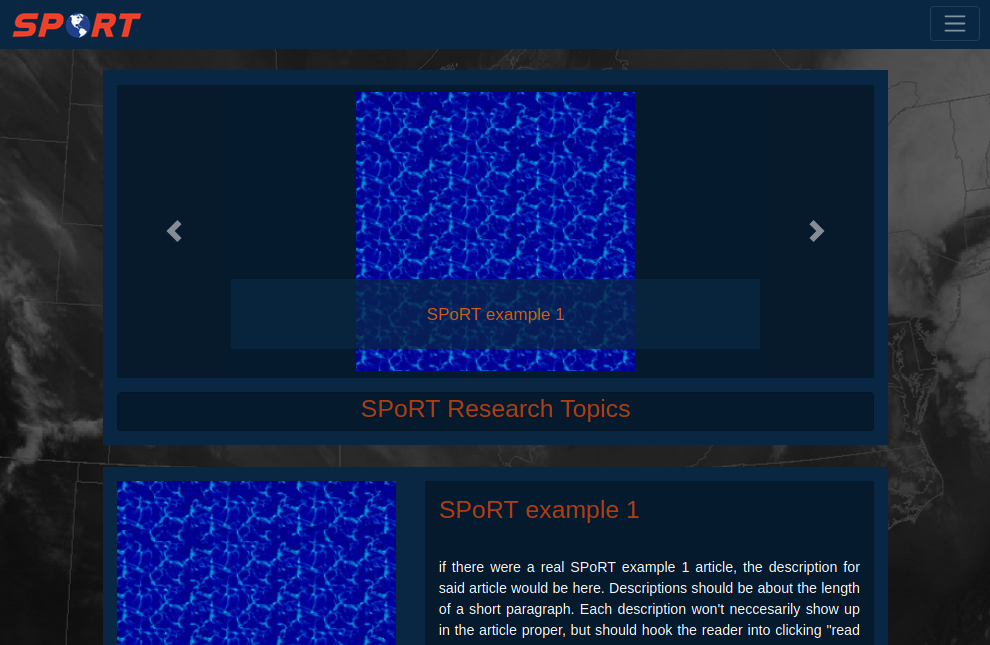
\includegraphics[width=.55\linewidth]{./figures/website_ss.png}
	\caption{SPoRT blog frontend concept}
	\label{concept} %(to reference in the future text)
\end{figure}

% --------------------------------------------------------------------------------------------------------

\section{Document 1: Software Design Documents}

\subsection{Audience}

The Software Design document will be the bulk of the SPoRT blog site documentation suite, written for future administrators of the SPoRT website and developers who wish to make changes to the website in the future. For this reason, the language of the design document will be far more technical than the other documents.

\subsection{Scope}

The software associated with the blog is split up into frontend, backend, and publishing packages by design, and as such the software design document will be divided into the same three categories. For each category, the design document will provide an abstract introduction to the function of the package, a detailed outline of the individual program modules within each package, and a series of diagrams and descriptions of the whole project at varying levels of abstraction. Documentation of individual modules contained within a package will include very detailed API information of the module as well as use cases, design philosophies, and solutions to any common issues that a programmer might encounter with the module. Much of the substance of the software design document will take the form of diagrams such as flow charts accompanied by explanatory text.

\subsection{Methodology}

Information contained in the software design document will primarily be collected in the process of designing and developing the programs themselves, however many design philosophies employed by the developers will be supported by programming standards and third-party research (accessibility research and object-oriented standards, for example).

\subsection{Qualifications}

As the primary designer and developer of the backend and publishing system of the blog site, as well as a team member for the front-end development of the site, I have a substantial understanding of the principles used as well as the actual implementation of the project. I will be able to create complete, accurate, and detailed text and diagrams for the software design document.

\subsection{Resources}

The following resources will be required to develop an effective software design document.

\begin{itemize}
	\item{Access to the full program suite of the blog frontend, backend, and publishing system.}
	\item{UML-like diagram development tool (I will be using inkscape).}
	\item{Computer and reliable typesetting software (\LaTeX).}
\end{itemize}


\newpage
% --------------------------------------------------------------------------------------------------------

\section{Document 2: Usability Test Report}

\subsection{Audience}

The usability test report will be tailored towards the developers of the front-end of the blog website. When developing a website, it is often difficult to get a sense of the issues users will encounter while navigating the website, using forms, or reading articles. The usability test report can help illuminate these problems so that the developers can find solutions prior to releasing the website to the public.

\subsection{Scope}

The usability test report will provide metrics on the usability of article sorting functions and forms (such as rating systems and comments), and on the navigability of the website on the whole on both mobile and desktop devices. In order to help minimize the amount of time and effort required to navigate and sort articles, metrics will include time taken to find an article, number of clicks required to preform a function, and subjective difficulty. This information will help the website developers design the blog so that is visually intuitive and easy to use.

\subsection{Methodology}

The framework currently used by blog developers (Bootstrap 4) makes the user experience of interacting with the blog website from a mobile device very practically different from interacting with it via a desktop computer. In order to effectively model the general user experience I will perform the following tests independently on both mobile and desktop devices using unique volunteers for each test.

\begin{enumerate}
	\item{\textbf{Navigation -} Ask user to find an article published on a specific date; record time and number of clicks required to complete task.}
	\item{\textbf{Forms -}  Ask user to get the RSS address of the website; record time and number of clicks required to complete task.}
	\item{\textbf{Sorting functions -} Ask user to prompt the website to display a specific category of articles (i.e. NUCAPS-related articles from March, 2019); record time and number of clicks required to complete the task.}
\end{enumerate}

\noindent
After all the tests, the volunteer will be asked to provide comments on the whole website.

\subsection{Qualifications}

As one of 2 web developers working on the SPoRT blog project, I have an understanding of the website's potential shortcomings, and will know how to make effective changes based on the information gathered by the usability tests.

\subsection{Resources}

The following resources will be required to develop an effective usability test report.

\begin{itemize}
	\item{6 volunteers (3 for mobile user testing, 3 for desktop user testing).}
	\item{1 mobile device and 1 desktop computer, each with a standard web browser.}
	\item{Timekeeping device and tables for recording time, clicks, and comments.}
	\item{Computer and reliable typesetting software (\LaTeX).}
\end{itemize}

% --------------------------------------------------------------------------------------------------------

\section{Document 3: Publishing How-To}

\subsection{Audience}

The publishing ``how-to'' document will be written for NASA SPoRT researchers who will be able to publish articles to the blog site. Researchers will need to interact with a command-line client (developed as a component of the publishing system in the software suite) which will allow them to easily publish to the website from any remote machine. Since some researchers may not have much experience using interfaces like this one, the publishing ``how-to'' document will assume very little technical experience or background knowledge, and will be act as a step-by-step walkthrough of the publishing process.

\subsection{Scope}

The publishing ``how-to'' page will be structured very much like a ``one problem, one solution'' document. In order to improve readability, the document will include graphics, screenshots, and will make use of formatting such as tables and lists.

\subsection{Methodology}

Information for the publishing how-to will be gathered by interviewing several of the research scientists who will be actively publishing articles when the blog site is finished. This should help me get a better sense of the amount of prior knowledge of CLI clients they generally have, and will help me discern which steps need to be especially well-described.

\subsection{Qualifications}

As a UAH contractor to SPoRT for more than a year, I've met many researchers who can provide context for the audience of the publishing how-to document, and can be potential candidates for user testing of the publishing client in conjunction with the publishing how-to-document (this may become a new component of the user test report if the publishing client software is finished on time).

\subsection{Resources}

The following resources will be required to develop an effective usability test report.

\begin{itemize}
	\item{Several researchers as volunteers for interviewing.}
	\item{Notetaking materials to make notes during interviews.}
	\item{Computer and reliable typesetting software (\LaTeX).}
\end{itemize}

% --------------------------------------------------------------------------------------------------------

%\section{Document 4: Website Tour}

%\subsection{Audience}

%\subsection{Scope}

%\subsection{Methodology}

%\subsection{Qualifications}

%\subsection{Resources}

% --------------------------------------------------------------------------------------------------------

\section{Timeline}

\begin{center}
	\begin{tabular}{ |l|l|c|c| }
		\hline
		\multicolumn{4}{ |c| }{Timeline} \\
		\hline
		Document & Tasks & Start & Finish \\ \hline

		\multirow{4}{*}{Software Design Documents}
		& API details                            & 5 & 7  \\
		& Module flow charts                     & 5 & 7  \\
		& High-level design philosophy           & 1 & 2  \\
		& Write and format document              & 8 & 12 \\ \hline

		\multirow{3}{*}{Usability Test Report}
		& Perform testing/data collection        & 0 & 4  \\
		& Aggregate and report data              & 5 & 7  \\
		& Write and format document              & 8 & 12 \\ \hline

		\multirow{3}{*}{Publishing How-To}
		& Interview researchers                  & 0 & 4  \\
		& Analyze interviews                     & 5 & 5  \\
		& Write and format document              & 8 & 12 \\ \hline
	\end{tabular}
\end{center}

\begin{center}
	{\footnotesize\noindent
	'Start' and 'Finish' in days since April 6 (first day after spring break). Project is due on day 21.
	}
\end{center}

\nocite{Brooke18}
\nocite{Melbourne15}
\nocite{Ceta20}

\printbibliography

\end{document}
